
\chapter{Experiments, Results and Analysis}
\label{experiments}
\epigraph{Experiment is the sole judge of scientific ``truth''}
{\textit{The Feynman Lectures on Physics, Introduction, Richard Feynman, 1961.}}


%%%%%%%%%%%%%%%%%%%%%%%%%%%%%%%%%%%%
\subsubsection{Extracting Information from the User Submitted Logs}
These variables of update probability and user install distribution can be extracted from the user submitted logs from the survey.
Initially, 31 logs where submitted, these logs were filtered to be APT logs, of more than 15 days long.
This resulted in 19 logs of between 23 and 277 days long to be processed.

An extract from one of these logs is shown in figure \ref{aptlog}.

\begin{figure}[htp]
\begin{center}
\begin{alltt}
\ldots
Start-Date: 2010-12-21 11:32:28
Install: libnet-daemon-perl (0.43-1), libhtml-template-perl (2.9-1), libdbi-perl (1.609-1build1), mysql-client-core-5.1 (5.1.41-3ubuntu12.8), libdbd-mysql-perl (4.012-1ubuntu1), mysql-server-5.1 (5.1.41-3ubuntu12.8), mysql-client-5.1 (5.1.41-3ubuntu12.8), libmysqlclient-dev (5.1.41-3ubuntu12.8), libplrpc-perl (0.2020-2), mysql-server-core-5.1 (5.1.41-3ubuntu12.8), mysql-server (5.1.41-3ubuntu12.8), libmysqlclient16-dev (5.1.41-3ubuntu12.8)
Upgrade: mysql-common (5.1.41-3ubuntu12.6, 5.1.41-3ubuntu12.8), libmysqlclient16 (5.1.41-3ubuntu12.6, 5.1.41-3ubuntu12.8)
End-Date: 2010-12-21 11:33:03
\ldots
\end{alltt}
\caption[APT log extract]{An extract of an APT log file}
\label{aptlog}
\end{center}
\end{figure}

In this log file a set of packages where installed and a few upgraded on the date 2010-12-21 11:32:28. 

These logs mainly describe the changes made to the system by APT, not necessarily what the user requested.
This is because APT may be used through another application, like semantic, to install or update the system.
As the criteria of APT is known, some information about the action the user requested can be inferred.

Given APT will never install or remove a component if the system is updated; 
if a package is upgraded but none are removed or installed then the user probably selected to update.
Also, if a package is installed, then the user requested a single package to be installed.
This second rule is assuming that only one package was selected, and not two at the same time.

Using these rules, each log is processed, and the variables of update probability and install distribution are measured.
These results are presented in table \ref{userlogvariables}.

As can be seen the lowest update probability is 0.05 or updating once every 20 days, and the highest was .96 so updating nearly every day.
The user who installs the least has a 95\% probability of installing nothing on a given day, where the most active user doesn't install anything on 32\% of days.

Some users have a probabilities of installing large amounts of packages in a single day, e.g. user 13.
This is due to some users have large amounts of activity installing, separated by low activity.

The correlation of these values is not explored in this relationship, here though the user who updates the least also installs the least,
and the user who updates the most, is the most likely to install one package on a given day.

These values can be assigned to their configuration variables in order to represent typical users and to answer different questions.


%%%%%%%%%%%%%%%%%%%%%%%%%%%%%%
%%%Previously we defined the conceptual model, this contains configuration variables used to simulate component system evolution
In the previous chapter the simulations conceptual model was defined.
This model contains variables used to configure the simulation of component system evolution.
To execute this simulation, first these variables and their assignments must be defined.
Before this is possible though, the component framework of the simulated evolution must be defined.
The component framework should contain enough information to the resolution necessary to create a realistic simulation configuration.

%%%Why Ubuntu was selected
The Ubuntu GNU/Linux distribution has been selected for this simulation as it fits these criteria.
This distribution contains a large and active repository of tens of thousands of components, with information at the necessary resolution.
Also, the open nature of its development and distribution makes it easy to find and access information.

%%%In this chapter\ldots
In this chapter the implementation of simulation using Ubuntu component framework is described.
This involves firstly describing the assignment and domain of configuration variables and the simulation processes.
Then the validation of this simulation, through comparing the results of a real system to that produced by the simulation, is described. 
Finally, we define specific question about component system evolution which are answered using this simulation.



\section{Questions}
This simulation has been defined and implemented in order to answer questions about component system evolution.
Defining the scope of these question is important, to stop the snowballing effect where getting answers can lead to more questions. 

The scope is defined through the core question of this research:

``What effect does using component resolution with different strategies have on system evolution?''.

This question has been broken up into three sub-questions,
\begin{itemize}
  \item Question 1 looks at strategies for updating
  \item Question 2 looks at different strategies for installing
  \item Question 3 looks at combining of installing and updating strategies
\end{itemize}

In this section these questions are broken into specific questions which are attempted to be answered though using our simulation.

\subsection{Question 1}
The most significant action for the evolution of a users system is through requesting to update its components.
This action can effect all components in the system, and can cause major changes in the way in a systems structure.
The strategy the user employs to update, involves how often they update, and what criteria they optimise their resolver for when updating.
As the installation is ignored in these questions, the install probability is set to 0 in the configuration.


\subsection{What are the effects of the extreme update strategies?}
%%%We answer this to find the range in which users can select their strategies
As described in chapter \ref{strategies}, the two main user sterotypes are that of the conservative user, who never wants to change their system,
and the progressive user, who wants to be most up to date.
These two extremes of this strategy are first measured to find the range in which all questions can be answered.

An extreme conservative user never wants to change their system, therefore their update strategy is to never update.
This will mean that there system will never update, and how fast they become out of date as this is what they are sacrificing is of interest.
This means that the criteria used for updating is unnecessary as it is never updated, and the user update probability will be 0.

On the other hand, an extreme progressive user will update every day with criteria where being up to date is the highest importance.
This will make this system change as much as necessary in order to have the newest components.
Specifically, the criteria that is used will be ``-uptodatedistance,-removed,-new'', and the user update probability will be 1.

\subsubsection{Results and Analysis}
The results are presented here.

How quickly the system with no updates goes out of date?
Does this represent most components, how fast they release?

Distribution of in out degree?
Does the system follow lehmans laws?
Does it become more complex (graph distributions).
if it doesnt, and we assume it to be true, either work has been done to make it less complex, or component system evolution does not follow lehmans laws.

\subsubsection{Conclusions}
These users represent only the most extreme users, and not the typical users strategy.
However, all other strategies exist between these two giving us a range of exploration in further questions.

\subsection{What are the effects of strategies that current users employed?}
%%%What is currently done in order to update a system
Through selecting a range of user submitted logs and extracting their update probabilities, a ``real'' users actions can be predicted.
These actions can then be simulated using different criteria from current resolvers.

The two resolvers that are being looked at are APT, the default Debian and Ubuntu resolver, and Eclipse P2, the Eclipse provisioning system.
As described in chapter \ref{strategies} the criteria for APT is ``-removed,-new,-uptodatedistance'', and for P2 it is ``-removed,-uptodatedistance,-new''.
The difference between these two resolvers is that APT is a more conservative resolver, where Eclipse P2 is more progressive.

Using these defined configurations 10 runs for each of 5 selected users where executed. 
These users where selected to represent a broad range of different update probabilities, and the amount of runs as different user probabilities will create different user actions.

\subsubsection{Results}
The results from this simulation are presented here:

The results when compared to the two extreme users presented in the previous question:

\subsubsection{Conclusion}
These results are interesting to note for two reasons. 
Firstly the difference over the time period when updating with either APT or Eclipse P2 is shown to be\ldots

When compared to the extreme users, there is a significant amount of area that the conservative.
How conservative users change their systems could be 

\subsection{What effect does a users update frequency have?}
%%%Why a user selects to upgrade at their update probability
A user will select to upgrade their system in order to increase the functionality of their system and to reduce risk of bugs being introduced.
These benefits are weighted against against the risk that it causes on their system due to the necessary change, to define the probability a user will upgrade on a given day.

%%%We have already explored the extremems and some real user probabilities, now we explore this as a range
The extremes of the users probability to upgrade, from updating every day to never upgrading, have been explored.
Also, some users have been simulated to see the effect on their update probabilities extracted from the submitted user logs.
Here, the update probability simulated over a range of possibilities, to find the relationship between it and the resulting systems probabilities.
For instance, what is the difference between a user who updates every day to one that updates half as much?

Specifically, the update probability is selected to be $[0,0.1,0.2,0.3,0.4,0.5,0.6,0.7,0.8,0.9,1]$,
selected as they cover the range of all update probabilities.  
The criteria will be the conservative ``-removed,-new,-uptodatedistance'', and progressive ``-uptodatedistance,-removed,-new''.
Each strategy (expect where the update probability is 1 or 0), will be executed 10 times to give a range of possible outcomes.

\subsubsection{Results}
The results are presented

\subsubsection{Conclusion}
The difference between updating 1 and .5 is insignificant. 

\subsection{What are the effects of only installing stable components?}
%%%We noticed something interesting
An interesting relationship was noticed when looking at the release cycles of different components;
components will often release a versions very close together then have long periods of not releasing.

%%%It might be caused by this
This effect may be caused by users of the package updating to the newly released version, 
finding and posting bug report to the maintain, who then quickly fixes the bug and releases a new versions to resolve the issue.
 
%%%Here is a real example of this happening
An example of this described situation is show in figures \ref{apachelog} and \ref{apachebug}.

\begin{figure}[htp]
\begin{center}
\begin{alltt}
apache2 (2.2.20-1) unstable; urgency=low

  * New upstream release.
  * Fix some regressions related to Range requests caused by the CVE-2011-3192
    fix. Closes: #639825
\ldots

 -- Stefan Fritsch <sf@debian.org>  Sun, 04 Sep 2011 21:50:22 +0200

apache2 (2.2.19-2) unstable; urgency=high

\ldots

 -- Stefan Fritsch <sf@debian.org>  Mon, 29 Aug 2011 17:08:17 +0200
\end{alltt}
\caption[Apache Changelog]{An extract from the apache changelog located on http://changelogs.ubuntu.com/}
\label{apachelog}
\end{center}
\end{figure}

\begin{figure}[htp]
\begin{center}
\begin{alltt}

Reported by: Takis Issaris <takis.issaris@uhasselt.be>
Date: Tue, 30 Aug 2011 16:09:01 UTC
Severity: important
Found in versions 2.2.9-10+lenny10, 2.2.16-6+squeeze2, apache2/2.2.19-2

\ldots

Package: apache2.2-common
Version: 2.2.9-10+lenny10

Yesterday evenings update broke our Apache server setup,
\ldots
\end{alltt}
\caption[Apache Bug Report]{Extract from the bug report \#639825, filed with Debian}
\label{apachebug}
\end{center}
\end{figure}

A summary of these evenets are:
\begin{enumerate}
  \item Apache developer Stefan Fritsch released a new version of their server, apache2/2.2.19-2, on 29 Aug 2011
  \item Takis Issaris upgraded to this version which broke their system on 29 Aug 2011
  \item Takis Issaris submits a bug report on 30 Aug 2011, where he and Stefan Fritsch discuss the causes
  \item On 04 Sep 2011 Stefan Fritsch releases a new version 2.2.20-1 that fixes this bug
\end{enumerate}


\subsubsection{Measuring the Effect}
By calculating the difference in days between each version of all components in the repository, 
over the dates of the simulation how often this situation occurs, where packages are quickly updated, can be measured.
In figure \ref{comeponentversionreleases} a graph is presented measuring the time difference between version releases.
 
\begin{figure}[htp]
\begin{center}
  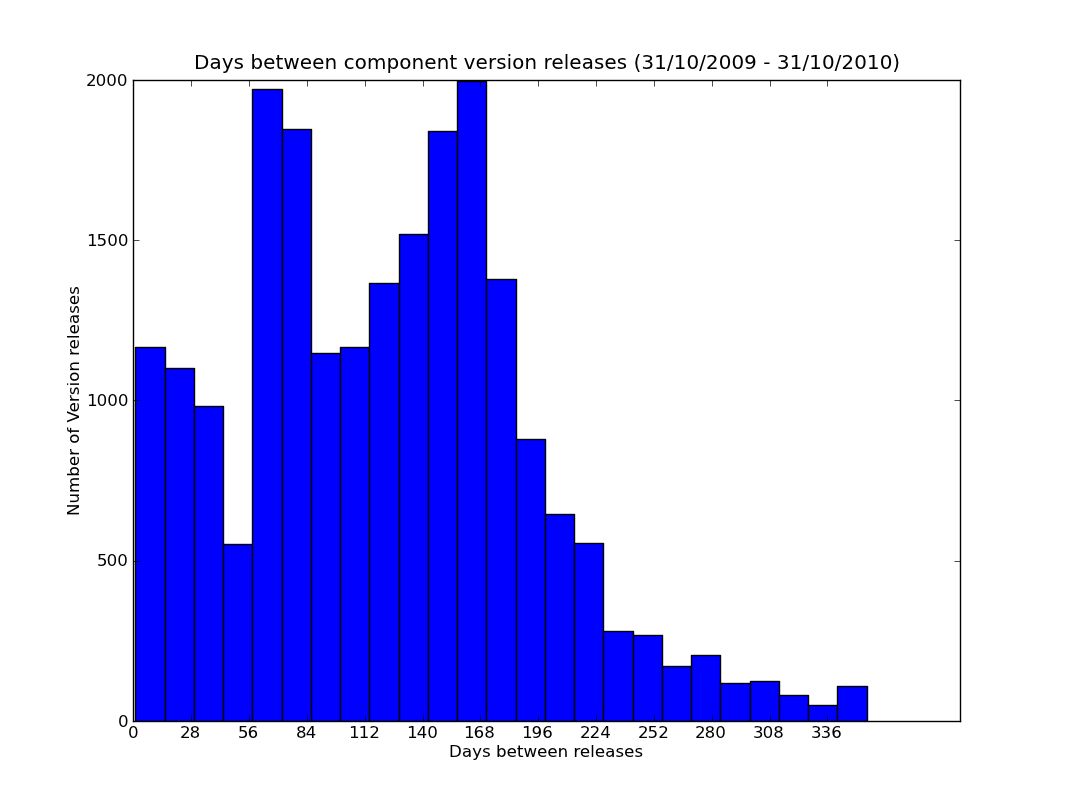
\includegraphics[width=\textwidth]{ubuntusimulationpics/versionreleasedistribution}
  \caption[labelInTOC]{Distribution of the releases of component versions between 31/10/2009 - 31/10/2010}
  \label{comeponentversionreleases}
\end{center}
\end{figure}

There are two points on this graph are noteworthy, firstly there is a large amount of components that release after 3 and 6 months.
Secondly there is a smaller but significant amount of components that have been released less than a month after the previous release.

The release of components after 3 or 6 month is probably due to the 6 monthly release cycle of Ubuntu.
Where individual components will release new versions for each Ubuntu release for it to be included.

\subsubsection{Effects of these releases}
%%%If this happens a lot, then these effects will happen
If this kind of release happens frequently to components in a repository, it causes much more change for a progressive user,
and standard strategies leave both conservative and progressive users vulnerable to the possible bug.

%%%A progressive user will experience a great deal more change with little benefit
The main effect of this kind of release causes to a progressive user is their system will go through more changes with little benefit.
As a progressive user will update frequently, it means they may upgrade to each release of a component.
As the time between the releases are so close to each other this only introduces more risk, and has little benefit for the system.

%%%Both types of users are vulnerable if the bug effects them
Another problem caused by this type of release is that if the bug effects the system, conservative users as well as progressive users are vulnerable.
Conservative users, although they update less frequently do update sometimes.
The time in which they update could be between one of these releases and then the bug can be introduced into their system, 
causing them to update once more, maybe introducing another bug.


\subsubsection{Criteria}   
The effects caused by these components that release soon after, i.e. within a month, of a previous release can be mitigated by taking into account when a component was released.
This criteria will then wait a certain amount of time once a package has been released, ensuring that no more releases are coming.
This idea is called ``Stable Version'', the main parameter that is required is the time in which to wait for a package to become stable.

This stable release criteria is defined as a hard constraint that can be added to a users update criteria.
%%%TODO This constraint is added, though it is not a criteira, TODO if there is only one package that has been released recently and asked to be installed will cause conflict

To test this criteria, to see if it reduces the effects of a set of user values is selected from the logs and extremes to build sets of user actions.
Through altering our progressive and conservative criteria to include the stable version criteria a range of values for the parameter of stable version is tested and measured for performance.
The criteria are altered to ``-stableversion(N),-removed,-new,-uptodatedistance'' and ``-stableversion(N),-uptodatedistance,-removed,-new'' where N is a number from a selected range.

\subsubsection{Results}
Compare against extreme and normal update distances.

\subsubsection{Conclusions}
The addition of the stable version criteria is shown to improve both the conservative and progressive user criteria.

It also shows that updating daily with a large stable version parameter is more conservative with better metrics than updating less frequently with no parameter.

\subsection{How do major releases effect component evolution?}
A release of a component system is a milestone in the system and repository.
It involves the cooperation of many parties, including the component systems managers, and the component developers.
This usually has many formal aspects to it, in Ubuntu there is an official schedule which is followed, an example shown in figure \ref{ubuntuSchedule}.

\begin{figure}[htp]
\begin{center}
  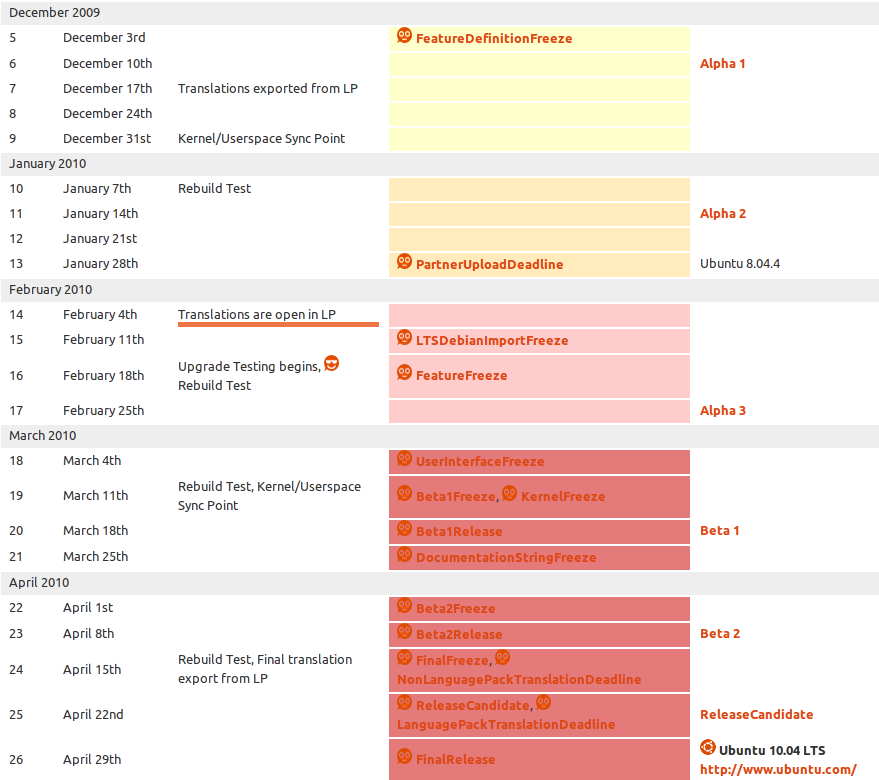
\includegraphics[width=\textwidth]{ubuntusimulationpics/ubunturelease}
  \caption[labelInTOC]{The Ubuntu release schedule from https://wiki.ubuntu.com/LucidReleaseSchedule accessed 6/3/2012}
  \label{ubuntuSchedule}
\end{center}
\end{figure}

This schedule involves multiple releases assuring quality of the final version, 
and freezes on different aspects of the components and system to assure that they do not change once the required quality has been found.


The consequences such schedules have on a repository is can be measured through comparing the activity of components added to the repository when compared to the different Ubuntu releases.
The amount of components added to the repository in relation to four different releases can be seen in figure \ref{ubuntureleases}.

\begin{figure}[htp]
\begin{center}
  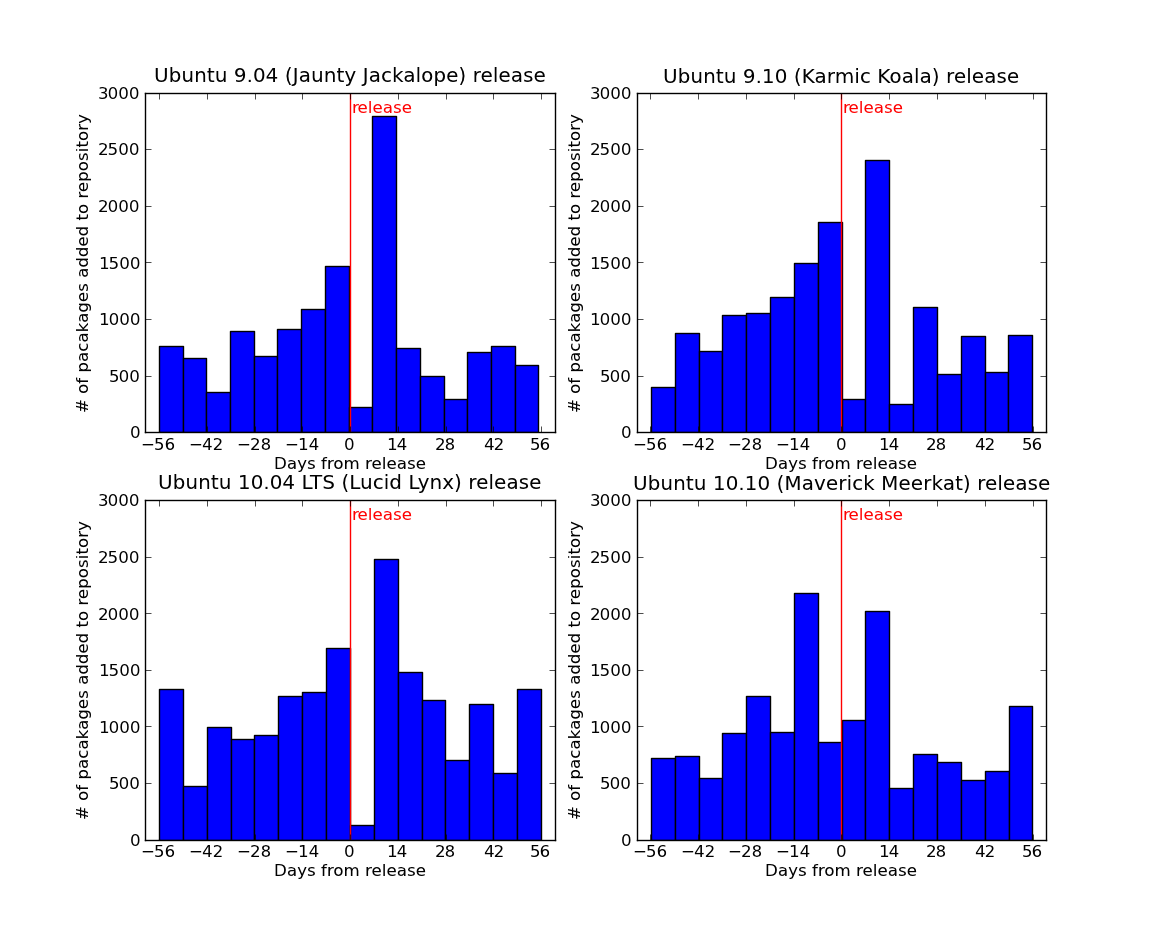
\includegraphics[width=\textwidth]{ubuntusimulationpics/releasedatepacakges}
  \caption[labelInTOC]{The amount of packages added to the repository in relation to the Ubuntu releases}
  \label{ubuntureleases}
\end{center}
\end{figure}

Three patterns can be seen in this figure, a build up to a release, a break after a release and a massive addition of components about two weeks after.

The build up to the release of components being added to the repository is probably component developers adding their latest versions to be included in the new major release.
The break after the release, where there is significantly less components added to the repository, is likely an effect of the freeze on addition of comopnents, while the new release stabilises.

The massive addition of components usually two weeks after the release, is the most concerning aspect.
Likely it is either a situation described previously where developers are receiving bug reports and adding fixes, 
or developers adding components that were unable to be added due to the freezes imposed on the repository. 

This leads to the question of how do these releases effect the evolution of a component system, because clearly they effect the repository.

\subsubsection{Experiment}
The simulations configuration is defined to execute over the Ubuntu 10.04 (Lucid Lynx) release.
Therefore, this is used to identify some of the effects that occur due to major releases in a repository.
There are some difference to reality that must be defined, firstly   

The previously defined experiments are now analysed with a closer eye on this period before and after a release, to analyse the effects on different criteria.
Specifically, the changes made to find if the changes increase in relation to the release date, and 

\subsubsection{Results}
The changes made to the system around the release date can be seen to increase significantly.

The changes made using the stable criteria, are delayed, but also less as it waits for the system to stabalise.

\subsubsection{Conclusion}
Major releases effect the evolution of a component systems.

This effect is felt mostly by users the update often and those that update progressivly.

The stable criteria as defined mitigates some of this effect of this system by waiting for the components to stabalize in their changes.

% \subsection{What is the effect of updating for while satisfying maximising recomends satisfaction?}
% As well as their explicit dependencies, components can define dependencies that they recommend should be installed.
% These components are usually what has been tested and are likely to interact with little friction with other components.
% Therefore, by satisfying these recomendation the system should be functional, though these recomendation may conflict with other users criteria.
% 
% Installing recommended pieces of software may duplicate functionality in  
% 
% Testing how the maximising the recomendations impacts the evolution of the system using the three 
% 
% Specifically, 10 runs for each of 5 selected users where executedusing the a
% conservative criteria ``-removed,-new,-unsat\_recommends,-uptodatedistance'', a progressive criteria ``-unsat\_recommends,-uptodatedistance,-removed,-new''
% and a mixed criteria ``-removed,-unsat\_recommends,-uptodatedistance,-new''.
% 
% \subsubsection{Results}
% Graphs of system size, system change are compared to the typical P2, APT and extreme progressive crtieria.
% 
% Life cycle, clearly the first update will hurt the most.
% 
% Show the trade offs.
% 
% 
% \subsubsection{Conclusion}
% Installing with recommendation may be prefered to increase stability, though it significantly increases the amount of change in a system, mostly at the begning.

\subsection{Graph metrics to lower change?}
The selection of the newest version is selected as it is presumed that the highest version is the best in the range of possible versions.
Graph metrics can measure the amount a component can be potentially be used.
However, given that the repository is always changing and newer versions are always added, the relationship between these metrics and their components,
is first needed to be studied in order to access this hypothesis.

%%%TODO
First we explore the way in which these values change over versions of components, because if it is linear it will not work.
If the value always increases over versions then the latest version will always be installed,
If the value always decreases then the least updated version is always installed, either of which can be much more easily calculated.

\subsubsection{Results}
Results from graph metrics that can be used.
Given a change, the number of components that depend on the changed components can be measured.
This could be described as the set of components that may through an error given a certain change.
If this is lower than using other conservative criteria this would be a sucessful use of criteira.

\subsection{What are the effects of a typical installation criteria?}
When a component is installed into a system the criteria is always conservative as the installation action is meant to change only parts of the system related to the selected components to install.
For instance, if the install criteria was progressive like ``-uptodatedistance,-removed,-new'', it would update the system when it installed, which is not its goal.

The extent at which the installation criteria is conservative can be altered per user.
The most conservative criteria criteria as described in \ref{strategies}  is ``-changed,-uptodatedistance'', this will only change a package if necessary and try to install uptodate versions.
The least conservative criteria that a user may want is ``-removedcomponent,-uptodatedistance,-changed'', this will first minimise removing any component from the original system,
then select uptodate components, finally minimising change.

Installation distributions can be measured in two different dimensions, how many components per install, and how often they select to install.
This gives us four typical users; a user who installs very few components infrequently; 
a user who installs very few components often;
a user who installs many components infrequently,
and a user who installs many components often install many components often.

Creating such user distributions is a difficult problem, as it involves creating realistic user interactions, which is very difficult.
Therefore, 4 user install distribution from user submitted logs who subjectively meet these descriptions have been selected to represent the extreme users.
These are simulated with the above defined criteria, to analyse the effect on component evolution.

Given the significant randomness that is involved with the installation property, 30 different user action sets have been generated for each user.

%TODO look at how the top 100 components install effect the system, for different criteria, how many components they add, and what common components are added!

\subsection{Results}
The effects of using these install criteria, focus on the 

How much change does a typical install cause (also investigated in \citep{Jenson2010})

\subsection{Conclusion}
This criteria is difficult to 

\subsection{Effects of installing and updating of typical users?}
Throughout these questions, criteria for updating and installtion, for progressive and conservative users have been defined and studied for their impacts on component system evolution.
It is asked here what impact these have overall, when combined together and simulated.

Specifically, four users will be created that express the sterotypes of extreme and moderarte versions of progressive and conservateive users.
Then 4 user install distributions and update probabilities will be selected from the user submitted logs that represent these user types and be simulated with 30 different user action sets each.

With these typical users, the simulation is run.
\subsubsection{Results}
The results are presented specifically showing the two main goals of limited uptodate

\section{Summary}
%%%A list of the answers gained from the questions
